\newpage{\ }
\cleardoublepage

\chapter{Apéndice Capítulo 4}\label{append_04}

\section{Índices de inflamabilidad}\label{append:FI}

Con el fin de parametrizar los índices de inflamabilidad, modelamos la probabilidad de que una celda se haya quemado al menos una vez en el período y área de estudio definidos en el Capítulo~\ref{cap:patrones} (1999-2022, 24 años). Extrajimos los datos de una muestra al azar de 9194 puntos tomados en la porción quemable del área de estudio, restringidos a tener una distancia mínima entre ellos de 800 m. El modelo fue definido de la siguiente manera:

\begin{equation}
\begin{aligned}
    y_i &\sim \ \text{Bernoulli}(\theta_i) \\
    \text{logit}(\theta_i) &= \alpha_{v[i]} + \beta_{v[i]} \ (NDVI_i - \omega_{v[i]}) \ +\gamma_1\ E_i + \gamma_2 \ N_i + \gamma_3 \ S_i \\
    \\
    \alpha_v &\sim \ \text{Normal}(\mu_{\alpha}, \sigma_{\alpha}) \\ 
    \log(-\beta_v) &\sim \ \text{Normal}(\mu_{\beta}, \sigma_{\beta}) \\
    \text{logit}(\omega_v) &\sim \ \text{Normal}(\mu_{\omega}, \sigma_{\omega}) \\
    \\
    \mu_{\alpha} &\sim \ \text{Normal}(0, 10) \\ 
    \sigma_{\alpha} &\sim \ \text{Normal}(0, 5)\text{T}[0, ] \\ 
    \\
    \mu_{\beta} &\sim \ \text{Normal}(\log(100), 2) \\ 
    \sigma_{\beta} &\sim \ \text{Normal}(0, 2)\text{T}[0, ] \\ 
    \\
    \mu_{\omega} &\sim \ \text{Normal}(0, 5) \\ 
    \sigma_{\omega} &\sim \ \text{Normal}(0, 3)\text{T}[0, ] \\ 
    \\
    \gamma_k &\sim \ \text{Normal}(0, 10),\ \text{con } k \in \{1, 2, 3\}.
\end{aligned}
\end{equation}

\noindent $y_i \in \{0, 1\}$ indica si la celda $i$ se quemó o no en el período de estudio, $\theta_i$ es su probabilidad de quema, $E$ es la altitud, $N$ es el componente norte de la orientación ponderado por la pendiente (orientación norte, ver~\eqref{eq:FI}), y $S$ es la pendiente de la ladera. Las tres variables topográficas fueron estandarizadas para el ajuste, pero luego sus parámetros fueron transformados a la escala original de las variables. El subíndice $v[i]$ indica el tipo de vegetación $\in \{1, ..., 5\}$ correspondiente a la celda $i$, y numerados de acuerdo a la Tabla~\ref{tab:fi_params_veg}. Los parámetros asociados a los efectos de la vegetación ($\alpha$, $\beta$, y $\omega$) fueron estimados con previas jerárquicas para facilitar la estimación de los tipos de vegetación con pocos datos, como el bosque seco. Nótese que se forzó a que $\beta$ fuera negativo para que el efecto del NDVI fuera unimodal. El efecto de la pendiente ($\gamma_3$) no era de interés para calcular el índice de inflamabilidad por topografía (IIT), pero se incluyó para mejorar la estimación de los demás parámetros. El efecto de la pendiente se toma en cuenta de forma separada en el modelo de propagación, pero en ese caso, es un efecto direccional, ya que varía según la propagación ocurra cuesta arriba o cuesta abajo. En \eqref{eq:FI} los índices son escalados para que tengan media 0 y desvío 1 en el conjunto de datos usado para ajustar este modelo.

\begin{figure}[htbp]
  \centering 
  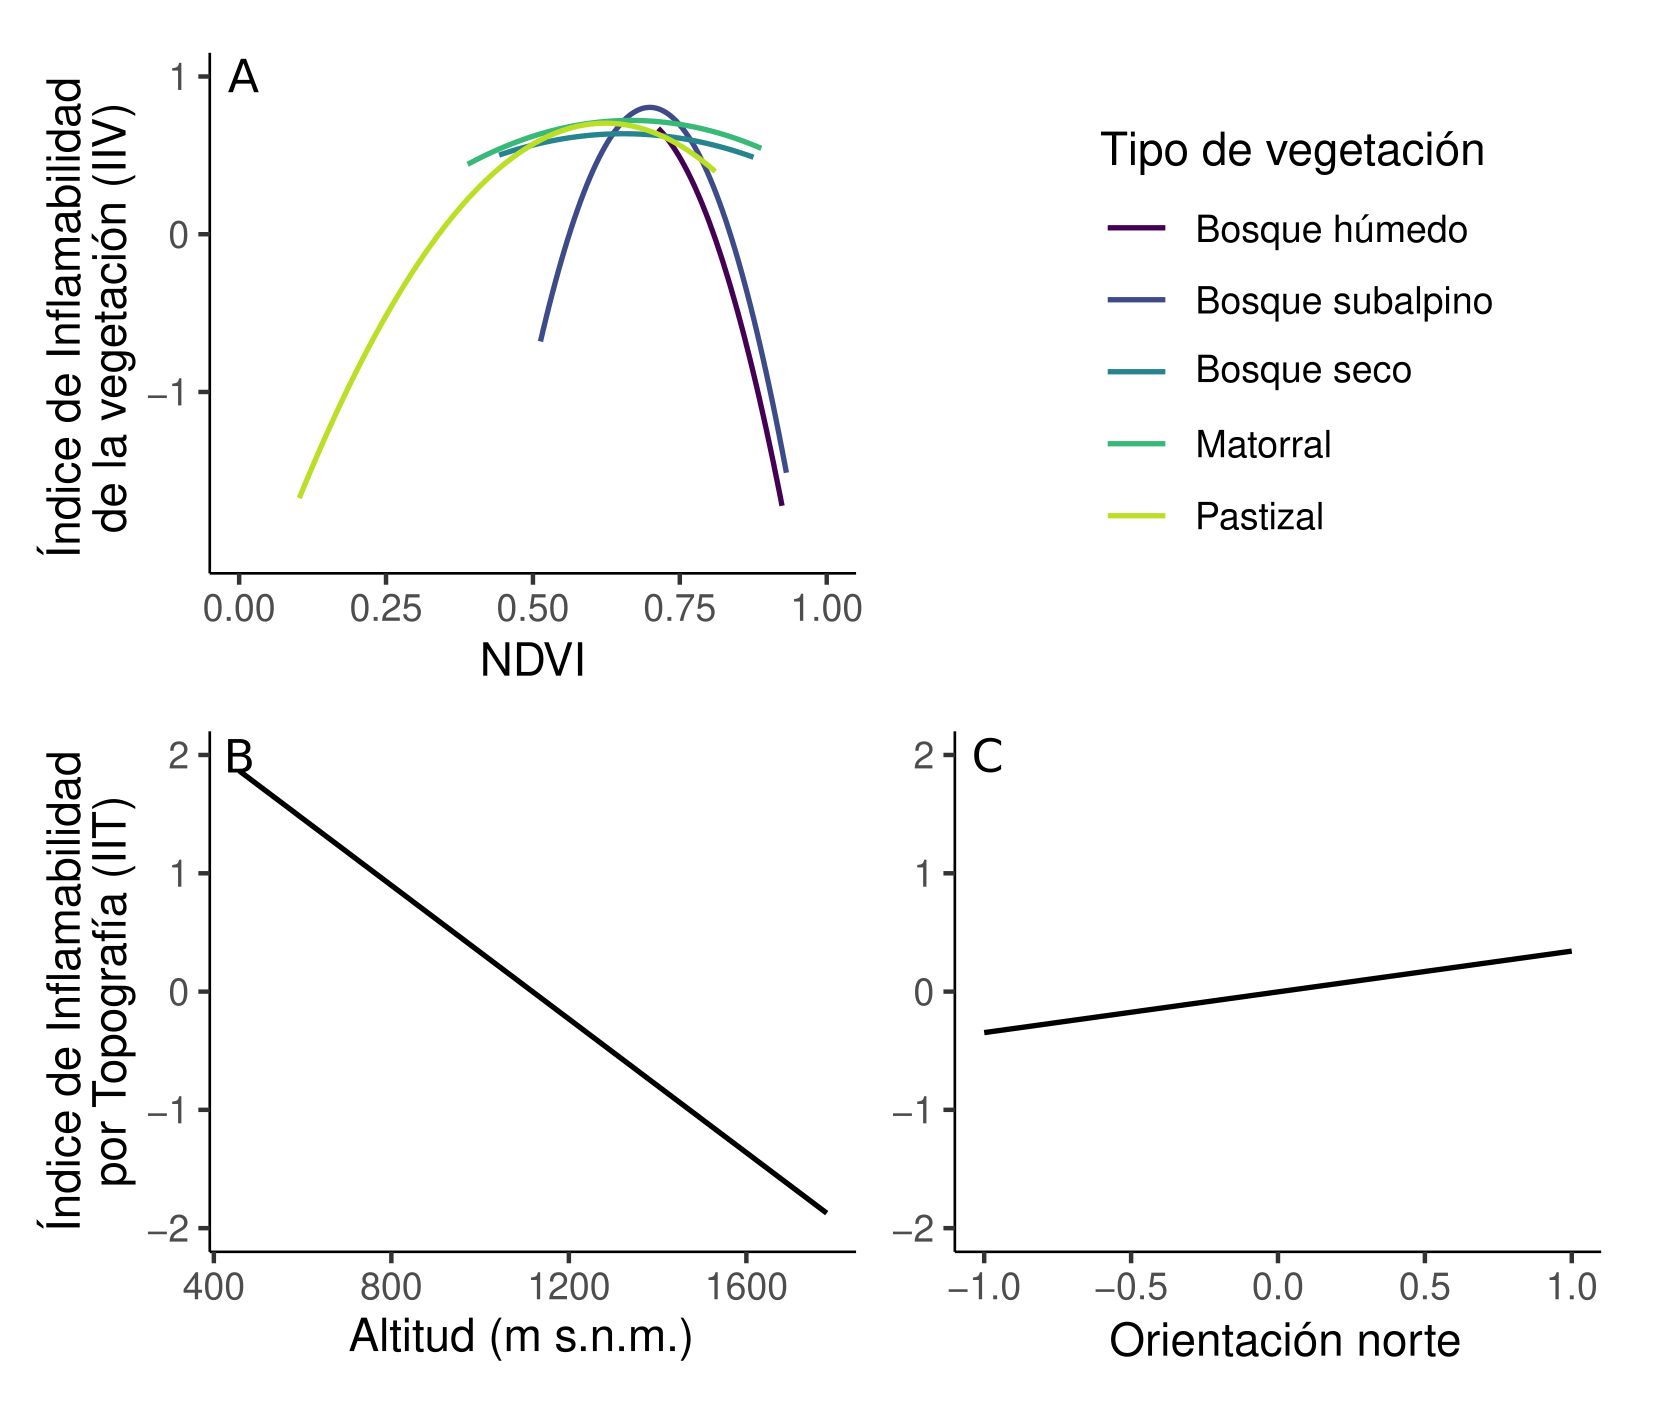
\includegraphics[width=14cm]{figuras/cap4/spread/flammability_indices.png}
  \caption{Índices de inflamabilidad en función de las variables que los componen, definidos en \eqref{eq:FI}.}
  \label{fig:FI}
\end{figure}

\FloatBarrier

\section{Proyecciones del régimen de incendios bajo cambio climático}\label{append:proj}

Los valores de FWI diario en su escala original diferían considerablemente entre las simulaciones de los modelos climáticos \citep{quilcaille2023FWI} y los datos basados en el reanálisis de ERA5 \citep{vitolo_era5-based_2020}, pero las anomalías quincenales de FWI presentaban una distribución muy similar. Sin embargo, dado que los datos y las simulaciones diferían en escala, las anomalías diarias de las simulaciones fueron calculadas a partir de la media y el desvío estándar del FWI basado también en simulaciones. Para cada realización de cada modelo climático y en cada escenario, las anomalías diarias de FWI fueron calculadas para los 3 períodos (1999-2023, 2040-2049, 2090-2099) de la siguiente manera:

\begin{enumerate}
    \item Definir período de referencia como la concatenación de la simulación climática para el final del escenario histórico (1999-2015) y el comienzo del escenario futuro correspondiente (2016-2023). 
    \item Calcular la media y desvío estándar de los valores diarios por celda en ese período.
    \item Estandarizar los valores diarios por celda en base a la media y desvío definidos en (2). Esto se hace para todos los días en los 3 períodos de interés: moderno, 2040s y 2090s.
    \item Promediar las anomalías diarias por quincena. 
\end{enumerate}

De esta manera, los valores se estandarizaron en base a la misma serie simulada. El período moderno de las simulaciones fue utilizado únicamente para evaluar cómo los modelos representaban el clima en dicho período, con el fin de ponderar los modelos adecuadamente. Para cada serie simulada de anomalías quincenales de FWI del período moderno (1999-2023) evaluamos su similitud con los datos basados en ERA5 mediante el índice de Bhattacharyya $B \in [0, 1]$, definido como:

\[
B(f, g) = \int \sqrt{f(x) \ g(x)}\ dx,
\]

\noindent donde $f()$ y $g()$ son las funciones de densidad de probabilidad. En este caso, estas densidades se obtuvieron por estimación basada en kernel utilizando los datos de ERA5 y las simulaciones. Previamente, remuestreamos los rasters a la resolución de ERA5 y recortamos todos al contorno del PNNH. Como cada modelo climático tenía un set de datos para el período moderno por cada escenario climático y realización, promediamos $B$ entre escenarios y realizaciones para obtener un único valor por modelo. En base a esta métrica definimos el peso de cada modelo como $P = \exp\{-[(1 - B) / 6]^2\}$ (no normalizado), para ponderar su aparición en las simulaciones de acuerdo a su capacidad de reproducir el clima observado. La Tabla~\ref{tab:climtable} detalla los modelos y realizaciones utilizados.

\begin{table}[htbp]
\centering
\caption[Modelos climáticos utilizados para las proyecciones.]{Modelos climáticos utilizados para las proyecciones. $B \in [0, 1]$ es el índice de similitud de Bhattacharyya entre las distribuciones de anomalía de FWI quincenal según el reanálisis de ERA5 o de las simulaciones climáticas. Los pesos se muestran relativizados al máximo para facilitar la comparación.}
\label{tab:climtable}
\small
\begin{tabular}{L{3cm} C{1.5cm} C{1.5cm} L{8cm}}
\toprule
Modelo & $B$ & Peso ($P$) & Realizaciones \\
\midrule
ACCESS-CM2 & 0.992 & 0.999 & r2i1p1f1, r3i1p1f1, r4i1p1f1, r5i1p1f1\\
ACCESS-ESM1-5 & 0.962 & 0.951 & r10i1p1f1, r11i1p1f1, r12i1p1f1, r13i1p1f1, r14i1p1f1, r15i1p1f1, r16i1p1f1, r17i1p1f1, r18i1p1f1, r19i1p1f1, r1i1p1f1, r20i1p1f1, r21i1p1f1, r22i1p1f1, r23i1p1f1, r24i1p1f1, r25i1p1f1, r26i1p1f1, r27i1p1f1, r28i1p1f1, r29i1p1f1, r2i1p1f1, r30i1p1f1, r31i1p1f1, r32i1p1f1, r33i1p1f1, r34i1p1f1, r35i1p1f1, r36i1p1f1, r37i1p1f1, r38i1p1f1, r39i1p1f1, r3i1p1f1, r40i1p1f1, r4i1p1f1, r5i1p1f1, r6i1p1f1, r7i1p1f1, r8i1p1f1, r9i1p1f1\\
CanESM5 & 0.979 & 0.986 & r10i1p1f1, r10i1p2f1, r11i1p1f1, r11i1p2f1, r12i1p1f1, r12i1p2f1, r13i1p1f1, r13i1p2f1, r14i1p1f1, r14i1p2f1, r15i1p1f1, r15i1p2f1, r16i1p1f1, r16i1p2f1, r17i1p1f1, r17i1p2f1, r18i1p1f1, r18i1p2f1, r19i1p1f1, r19i1p2f1, r1i1p1f1, r20i1p1f1, r20i1p2f1, r21i1p1f1, r21i1p2f1, r22i1p1f1, r22i1p2f1, r23i1p1f1, r23i1p2f1, r24i1p1f1, r24i1p2f1, r25i1p1f1, r25i1p2f1, r2i1p1f1, r2i1p2f1, r3i1p1f1, r3i1p2f1, r4i1p1f1, r4i1p2f1, r5i1p1f1, r5i1p2f1, r6i1p1f1, r6i1p2f1, r7i1p1f1, r7i1p2f1, r8i1p1f1, r8i1p2f1, r9i1p1f1, r9i1p2f1\\
CMCC-ESM2 & 0.980 & 0.987 & r1i1p1f1\\
EC-Earth3 & 0.984 & 0.993 & r1i1p1f1, r4i1p1f1\\
FGOALS-g3 & 0.989 & 0.997 & r1i1p1f1, r3i1p1f1\\
INM-CM4-8 & 0.978 & 0.984 & r1i1p1f1\\
INM-CM5-0 & 0.993 & 1.000 & r1i1p1f1\\
IPSL-CM6A-LR & 0.993 & 1.000 & r14i1p1f1, r1i1p1f1, r2i1p1f1, r3i1p1f1, r4i1p1f1, r6i1p1f1\\
MIROC-ES2L & 0.976 & 0.981 & r10i1p1f2, r1i1p1f2, r2i1p1f2, r4i1p1f2, r5i1p1f2, r6i1p1f2, r7i1p1f2, r8i1p1f2, r9i1p1f2\\
MIROC6 & 0.990 & 0.998 & r1i1p1f1, r2i1p1f1, r3i1p1f1\\
MPI-ESM1-2-HR & 0.947 & 0.905 & r1i1p1f1, r2i1p1f1\\
MPI-ESM1-2-LR & 0.951 & 0.919 & r10i1p1f1, r11i1p1f1, r12i1p1f1, r13i1p1f1, r14i1p1f1, r15i1p1f1, r16i1p1f1, r17i1p1f1, r18i1p1f1, r19i1p1f1, r1i1p1f1, r20i1p1f1, r21i1p1f1, r22i1p1f1, r23i1p1f1, r24i1p1f1, r25i1p1f1, r26i1p1f1, r27i1p1f1, r28i1p1f1, r29i1p1f1, r2i1p1f1, r30i1p1f1, r3i1p1f1, r4i1p1f1, r5i1p1f1, r6i1p1f1, r7i1p1f1, r8i1p1f1, r9i1p1f1\\
MRI-ESM2-0 & 0.831 & 0.358 & r1i1p1f1, r2i1p1f1, r3i1p1f1, r4i1p1f1, r5i1p1f1\\
\bottomrule
\end{tabular}
\end{table}

\FloatBarrier

\section{Efecto de la vegetación sobre la probabilidad de propagación en función del FWI}\label{append:spread-veg-effects}

Un aspecto relevante del modelo de propagación era cómo cambiaba el efecto del tipo de vegetación sobre la probabilidad de propagación con el FWI. Si bien el coeficiente asociado a la vegetación ($\beta_1$, IIV; Ecuación~\ref{eq:datamodel}) no varió en función del FWI (Fig.~\ref{fig:spread-params}B), la no linealidad de la función logística hace que el efecto de una variable sobre la probabilidad de propagación dependa también del efecto y del valor de otras variables, incluso cuando no hay coeficientes de interacción, como en nuestro modelo. Esto es relevante porque el FWI afectó a otros coeficientes de propagación, como aquellos regulando el efecto del viento y la pendiente ($\beta_3$ y $\beta_4$; Ecuación~\ref{eq:datamodel}; Fig.~\ref{fig:spread-params}Dy E). Si al aumentar el FWI el efecto del viento aumentaba lo suficiente como para llevar la probabilidad de propagación cerca de 1 (Fig.~\ref{fig:spread-curves}D), el efecto de la vegetación podría atenuarse, al menos considerando propagación a favor del viento. Para evaluar la posibilidad de esta interacción implícita, evaluamos cómo cambiaba el efecto del tipo de vegetación sobre la probabilidad de propagación en función del FWI, considerando los efectos del FWI sobre todos los parámetros de propagación. 

Para poder comparar los tipos de vegetación, fijamos la altitud en 900 m s.n.m. y la orientación en 90~° (implicando orientación norte = 0), fijando así el IIT (Índice de Inflamabilidad por Topografía). Para considerar en la predicción el efecto direccional de la pendiente y el viento sobre la probabilidad de propagación, considerando su variabilidad en el PNNH, muestreando 500 celdas de su zona quemable, utilizando el raster creado para la simulación de incendios, que contenía, entre otras variables, la velocidad del viento y la pendiente (Sección~\ref{cap4:data}). Para considerar el efecto de la pendiente tanto cuesta arriba como cuesta abajo, duplicamos el conjunto de celdas y fijando la pendiente en 0° en la segunda mitad (el modelo de propagación asume que la propagación cuesta abajo es igual que en llano; Ecuación~\ref{eq:datamodel}). 

Para comparar los tipos de vegetación necesitábamos obtener el IIV (Índice de Inflamabilidad de la Vegetación) para cada uno, con lo cual, requeríamos el NDVI. Como el NDVI varía en función de la topografía, calculamos su valor esperado para las condiciones topográficas analizadas (500 valores de pendiente, con altitud y orientación fijas) utilizando un modelo de NDVI, con un enfoque similar a lo expuesto en el Apéndice~\ref{append:cov}. Ajustamos un Modelo Aditivo Generalizado con distribución Beta para el NDVI  escalado a [0, 1], utilizando el mismo conjunto de datos con el cual se estimaron los parámetros de los índices de inflamabilidad (Apéndice~\ref{append:FI}). Incluimos como predictoras la pendiente, altitud y orientación en base a resultados del Capítulo~\ref{cap:patrones} (Fig.~\ref{fig:cap3-S07}). Con este modelo predijimos el NDVI a 900 m de altitud, con orientación este, y sobre todos los valores de pendiente muestreados, con el cual, calculamos el IIV para cada tipo de vegetación en todas las celdas muestreadas.

En base a la altitud y orientación fijadas, a los 500 valores de pendiente y viento muestreados (además de los 500 valores con pendiente fijada en cero), con sus respectivos IIV para cada tipo de vegetación, calculamos la probabilidad de propagación por tipo de vegetación a lo largo de una secuencia de FWI, promediando las predicciones a lo largo de las celdas muestreadas. De esta manera, las predicciones condicionan en valores fijos de altitud, orientación y tipo de vegetación y marginalizan sobre la distribución de velocidad del viento, pendiente y NDVI en el PNNH, asumiendo siempre dirección del viento a favor de la propagación. Además, las predicciones se calcularon marginalizando sobre los efectos aleatorios mediante simulación. 

El efecto del tipo de vegetación sobre la probabilidad de propagación (Fig.~\ref{fig:spread-veg-effects}A) se definió como el desvío absoluto medio a lo largo de los cinco tipos de vegetación, ponderándolos a todos por igual. 

\section{Propagación, resultados extendidos}\label{append:spread_results}

\begin{figure}[H]
  \centering 
  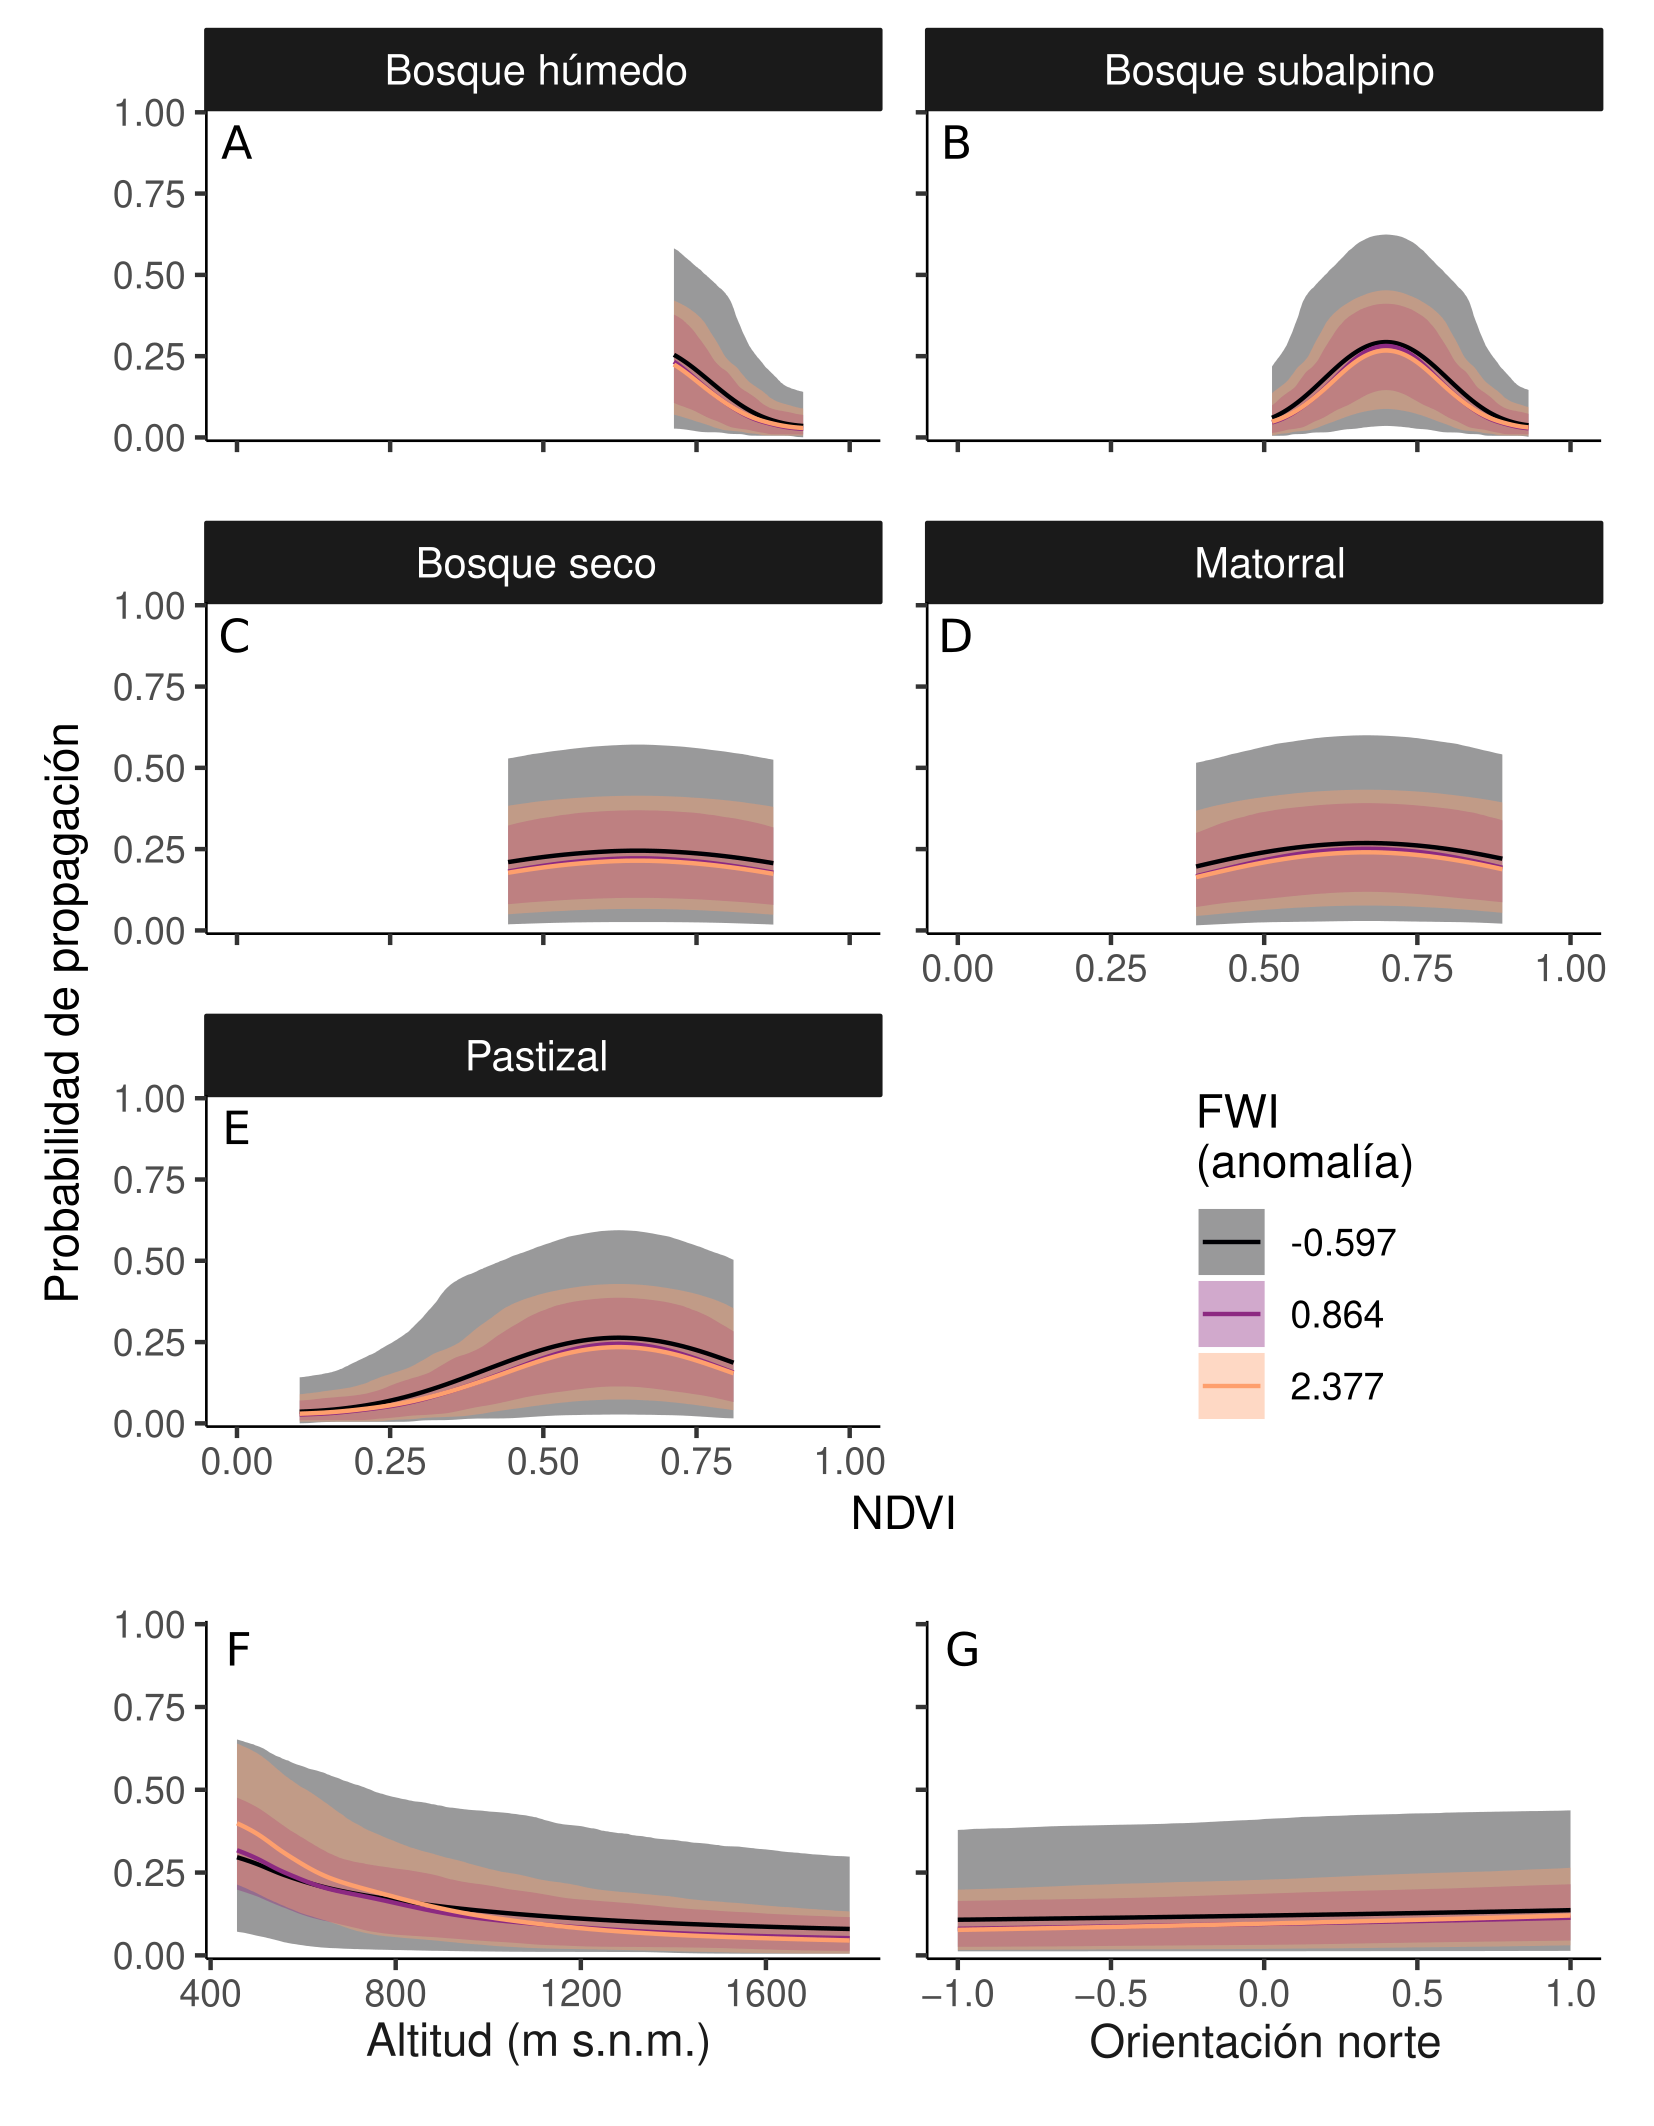
\includegraphics[width=14cm]{figuras/cap4/spread/spread_prob_curves_raw_x.png}
  \caption[Probabilidad de propagación en función del NDVI, el tipo de vegetación, la altitud y la orientación.]{Probabilidad de propagación en función las predictoras, descomponiendo los índices de inflamabilidad de vegetación y por topografía en sus variables crudas.}
  \label{fig:spread-curves-x}
\end{figure}

\begin{figure}[htbp]
  \centering 
  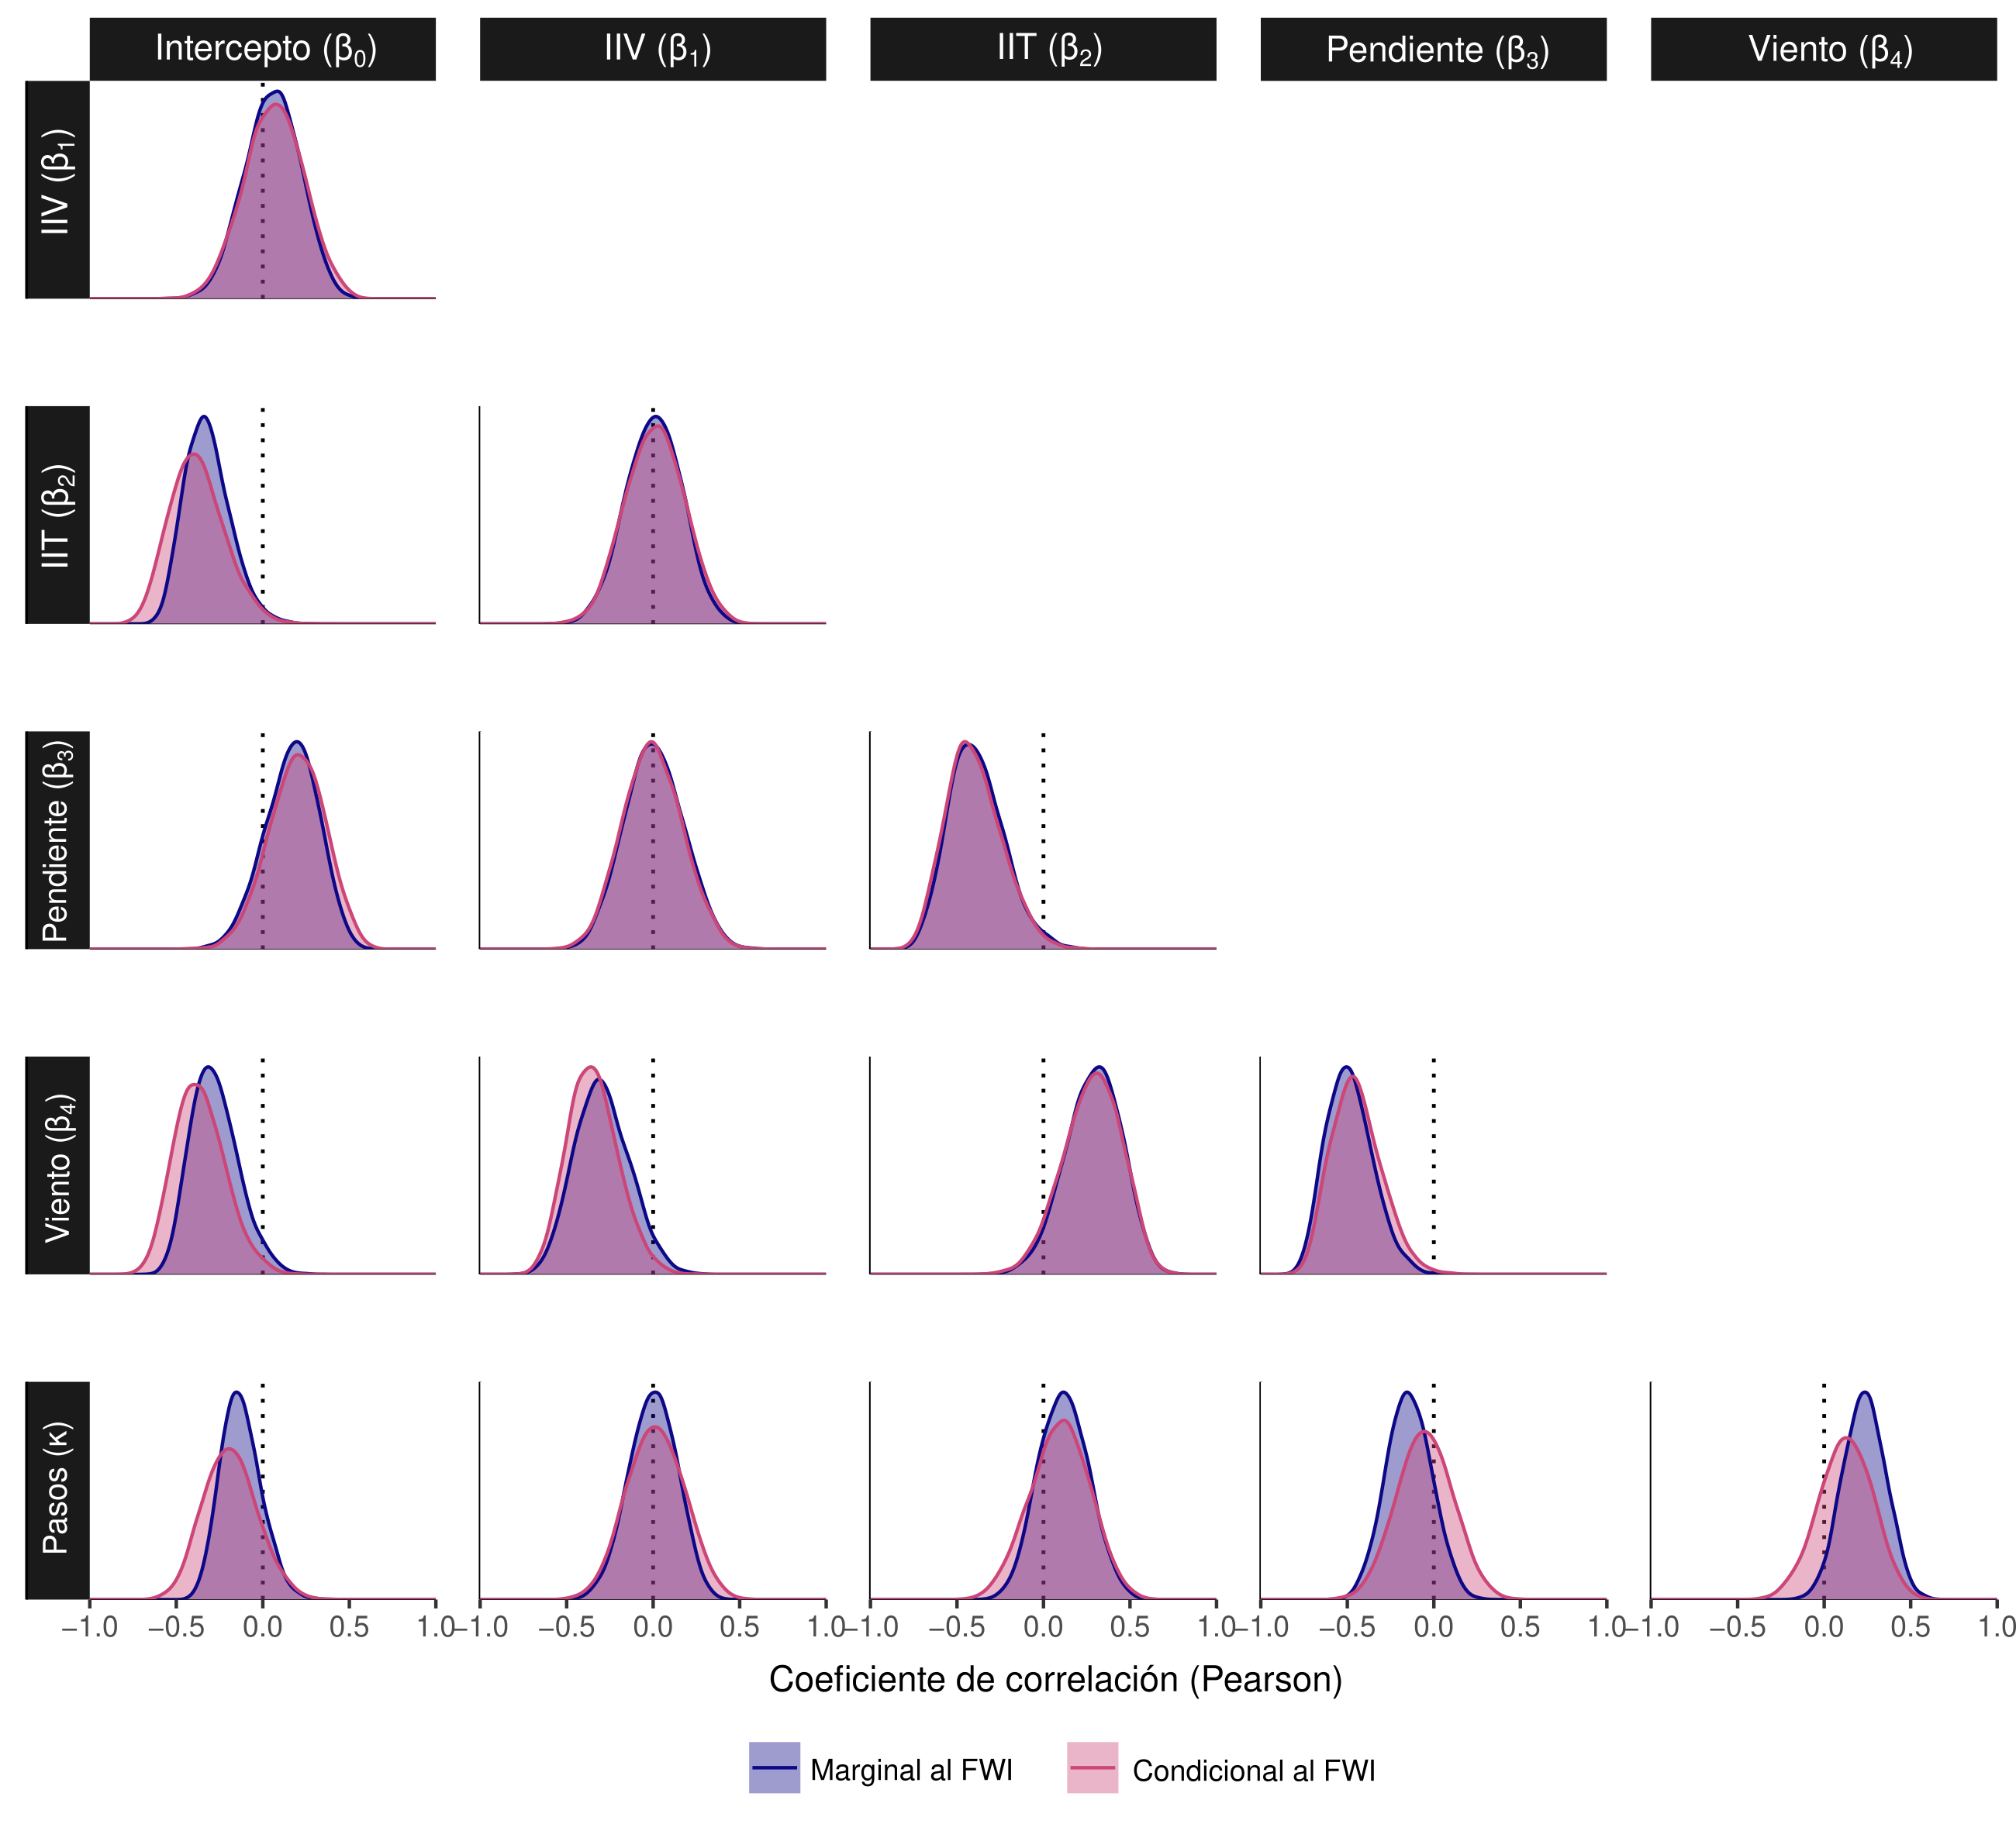
\includegraphics[width=\textwidth]{figuras/cap4/spread/pairs_plot_correlations_posteriors.png}
  \caption[Correlación entre los parámetros de propagación.]{Distribución posterior del coeficiente de correlación de Pearson entre cada par de parámetros de propagación, condicional o incondicional al FWI. Los coeficientes fueron calculados simulando valores de la Normal Multivariada ajustada. Las distribuciones condicionales al FWI fijan el FWI en la media de los datos de propagación, y representan la posterior de $\boldsymbol{\Omega}$ (ver Ecuación~\ref{eq:hier2}). La distribución incondicional al FWI incluye su efecto FWI: parámetros que son afectados de forma similar (diferente) por el FWI presentaría una correlación incondicional de mayor (menor) magnitud que la condicional.}
  \label{fig:spread-corr}
\end{figure}

\FloatBarrier

Las siguientes figuras muestran el ajuste del modelo de propagación. Como describimos en la sección~\ref{cap4:spread-model}, para cada incendio se estimó un vector de parámetros $\boldsymbol{\beta}$, el cual regula la propagación. Permitir que estos parámetros variaran entre incendios fue una forma de representar variables no observadas relevantes para el fuego. Por ejemplo, un incendio que fue apagado rápidamente por combatientes o por lluvia puede presentar un menor número de pasos ($\kappa$) que el promedio, y un incendio que propagó con elevada velocidad del viento puede presentar un efecto fuerte del viento ($\beta_4$). A su vez, a partir la variabilidad en $\boldsymbol{\beta}$ entre incendios y de cómo esta variabilidad se relacionaba con el FWI de cada incendio, estimamos una distribución de parámetros (Ecuación~\ref{eq:hier1}), que nos permite simular nuevos $\boldsymbol{\beta}$ para incendios hipotéticos. Para evaluar el ajuste del modelo comparar incendios observados con incendios simulados. Pero existen dos formas de hacerlo: (1) utilizar los \textit{parámetros ajustados} para cada incendio, o (2) simular nuevos parámetros de la distribución estimada (\textit{parámetros simulados}). Es esperable que en el primer caso los incendios simulados se parezcan más a los observados, en cambio, utilizando parámetros simulados estamos simulando incendios que difieren de los observados en las variables no observadas representadas por estos parámetros (e.g., velocidad del viento, combate, precipitaciones, etc.).

\begin{figure}[htbp]
  \centering 
  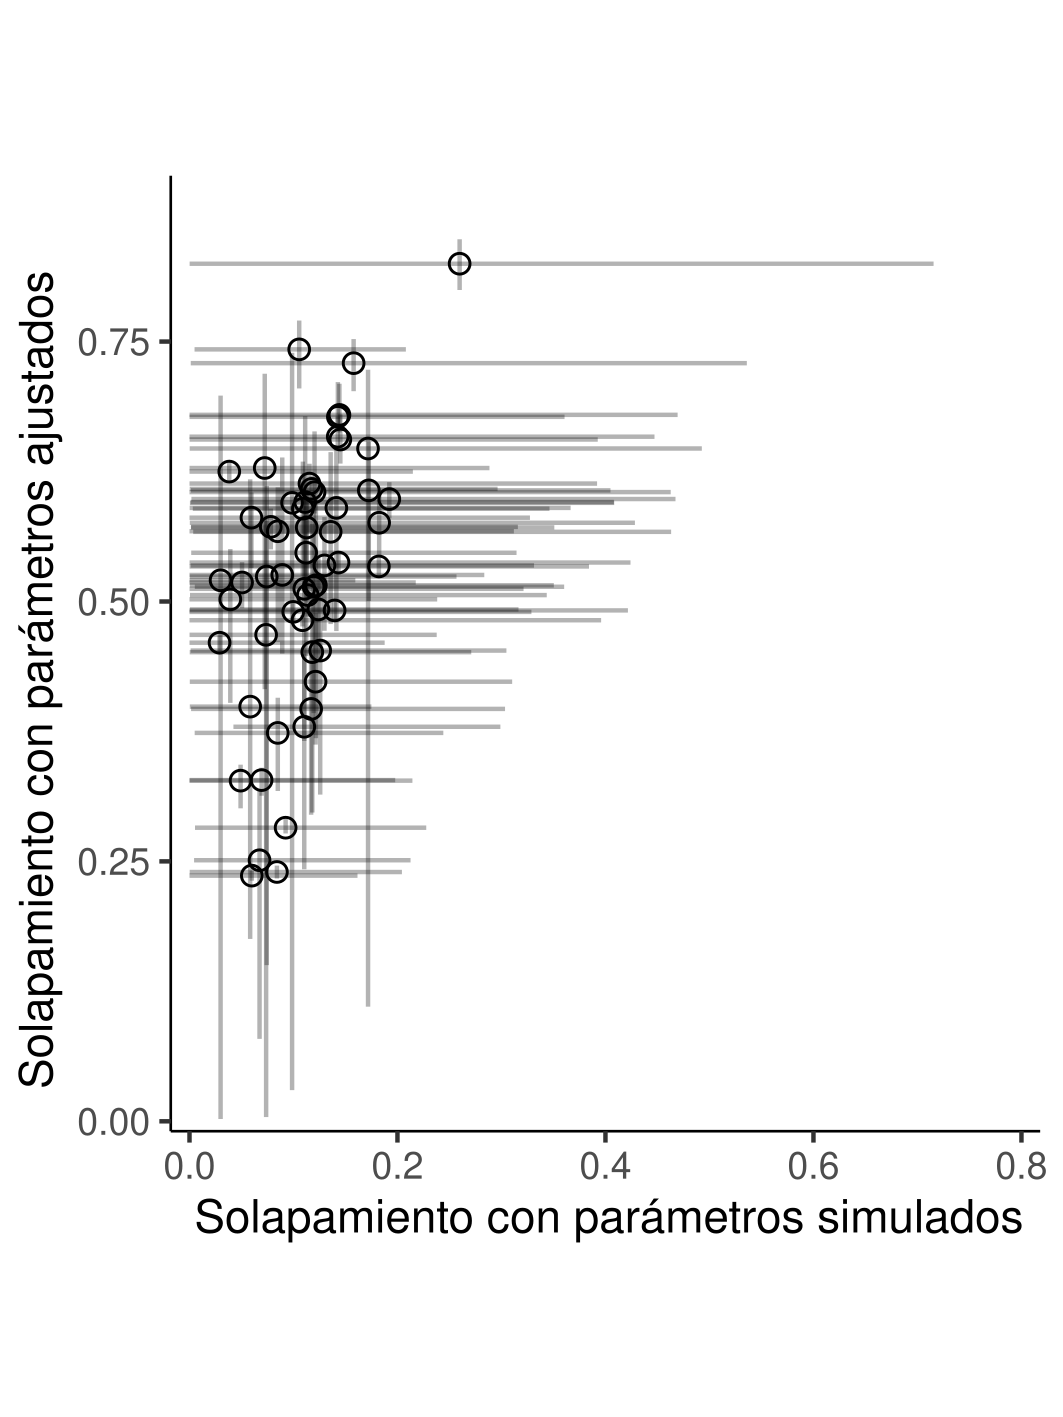
\includegraphics[width=9cm]{figuras/cap4/spread/overlap_fit_sim.png}
  \caption[Solapamiento espacial entre incendios simulados y observados.]{Solapamiento espacial entre incendios simulados y observados, utilizando los parámetros ajustados para cada incendio o simulando nuevos parámetros a partir de la distribución estimada. Los puntos y líneas indican la media y el intervalo de credibilidad del 95 \% de la distribución posterior del solapamiento, aproximada mediante 2000 simulaciones para cada tipo de uso de los parámetros e incendio.}
  \label{fig:spread-ov}
\end{figure}

\begin{figure}[htbp]
  \centering 
  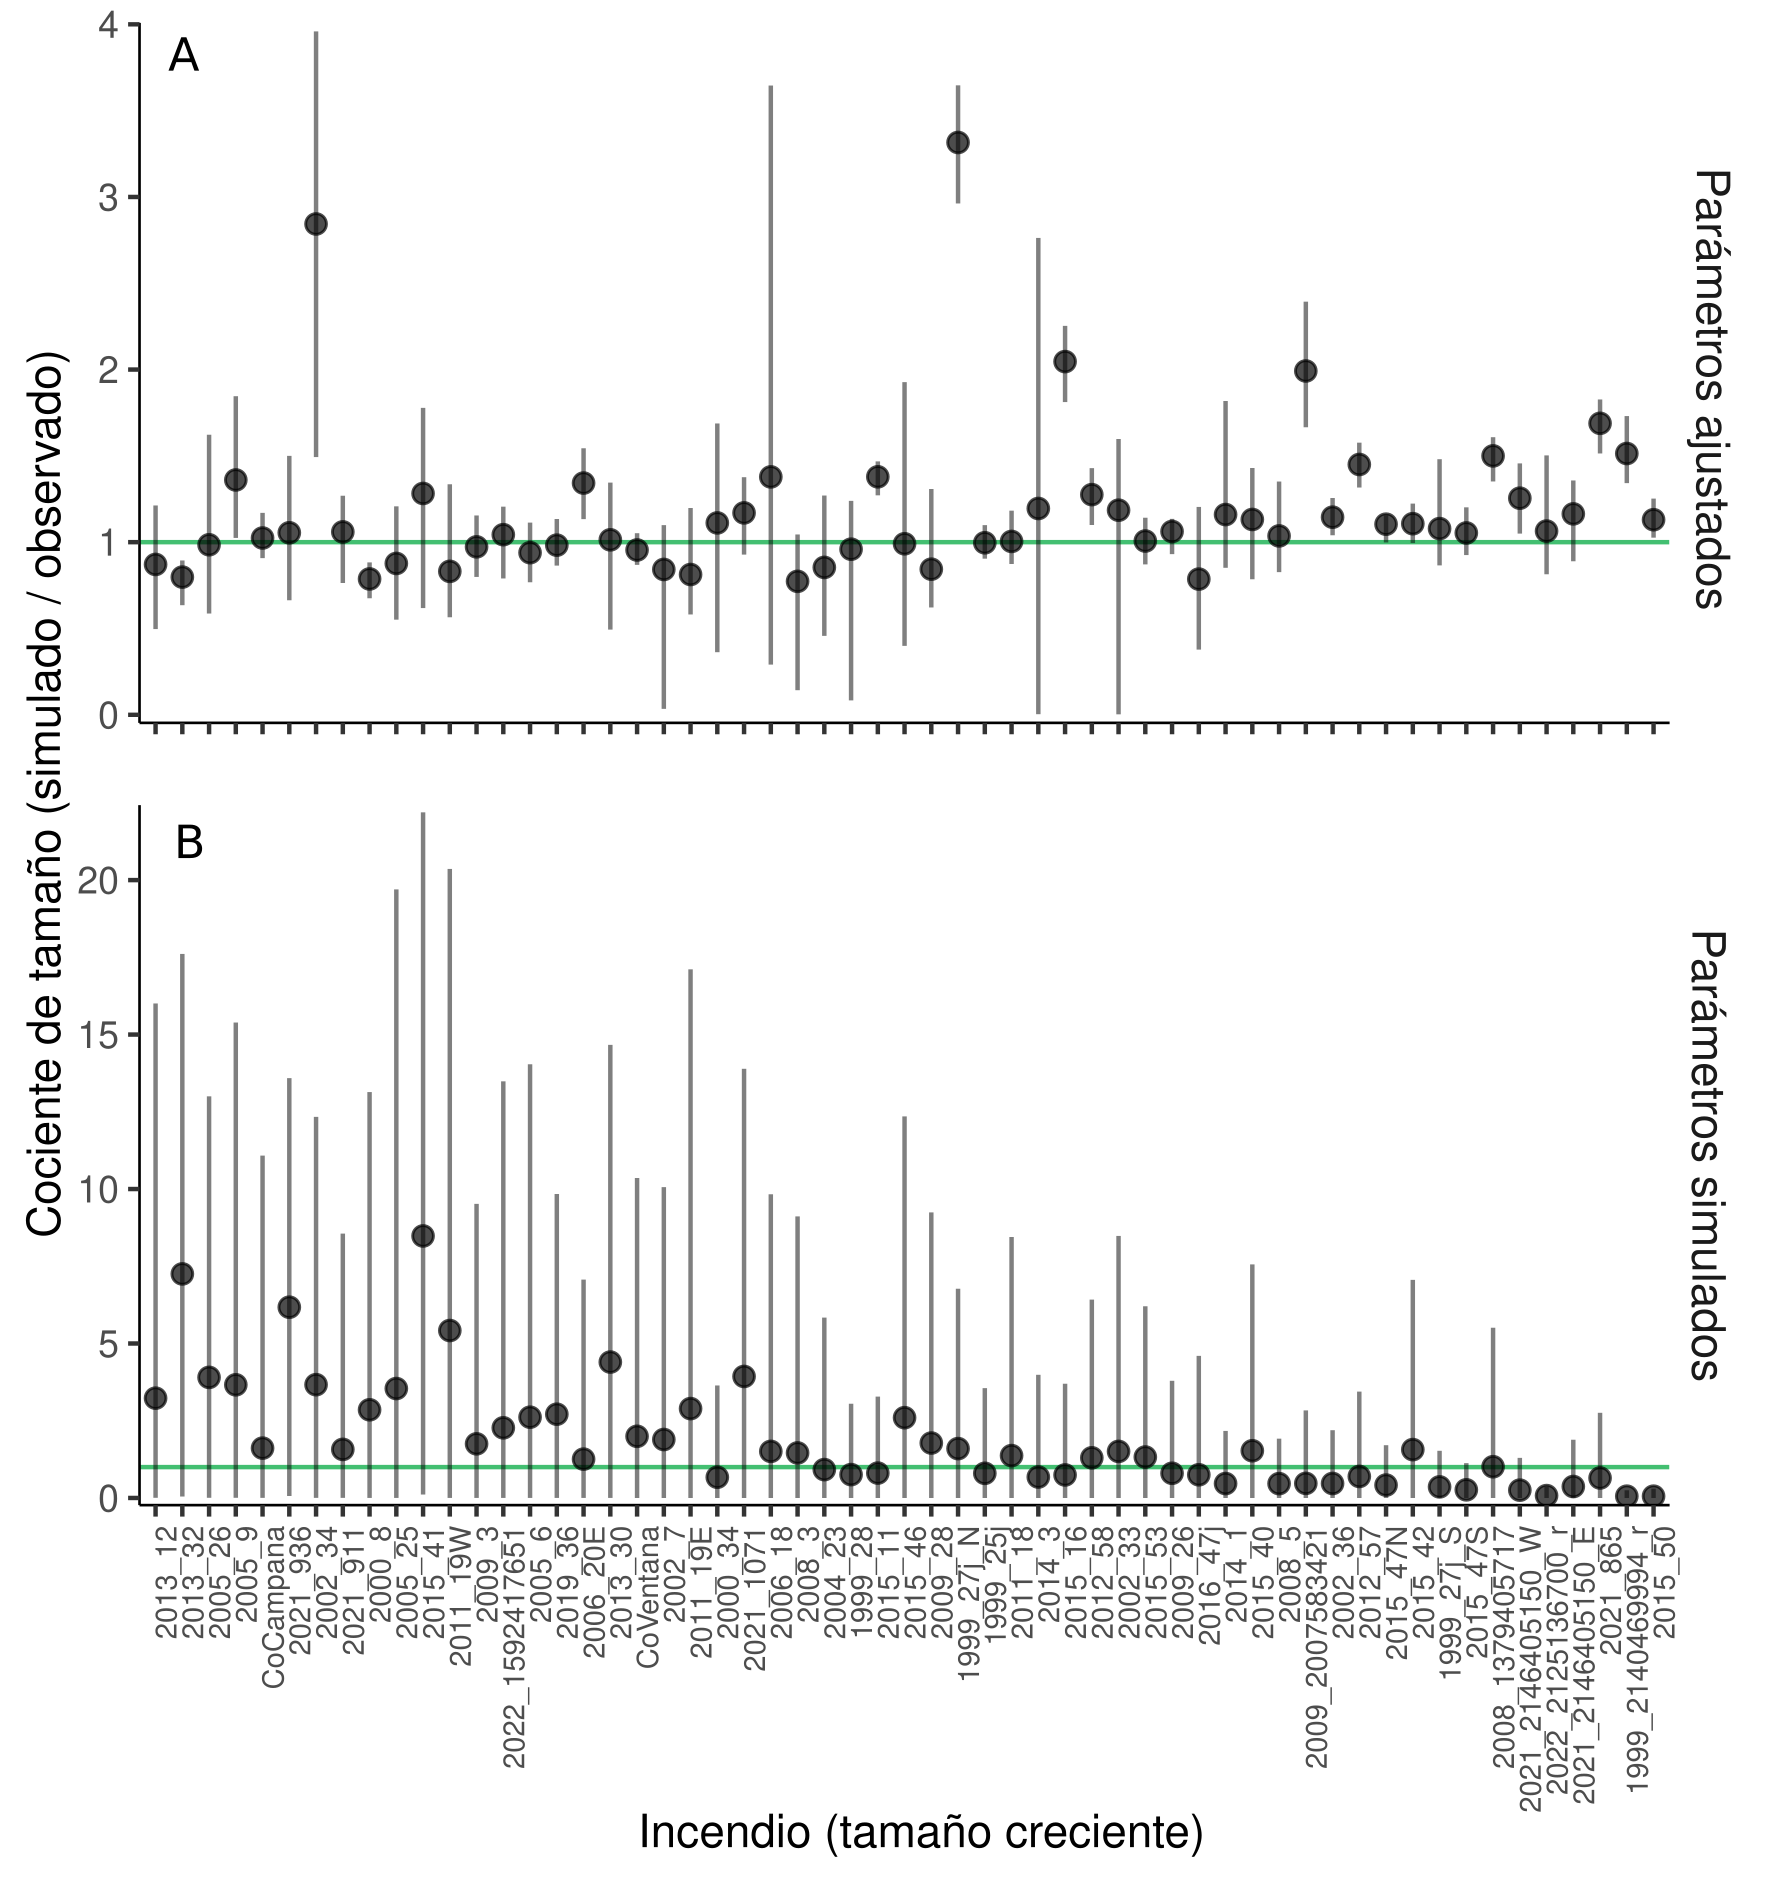
\includegraphics[width=15cm]{figuras/cap4/spread/quotient_sim_obs_fire_size.png}
  \caption[Cociente de tamaño de incendios simulados y observados.]{Cociente de tamaño de incendios simulados / observados, utilizando los parámetros ajustados para cada incendio o simulando nuevos parámetros a partir de la distribución estimada. Los puntos y líneas indican la media y el intervalo de credibilidad del 95 \% de la distribución posterior del cociente, aproximada mediante 2000 simulaciones para cada tipo de uso de los parámetros.}
  \label{fig:spread-q}
\end{figure}

\FloatBarrier

Si bien el modelo presenta un mal ajuste al usar parámetros simulados, nuestro objetivo no era desarrollar un simulador que pudiera predecir con precisión el avance del fuego en un incendio puntual, sino un simulador capaz de generar incendios similares a los que ocurren en nuestra área de estudio. Así, el mal ajuste observado al usar parámetros simulados no invalida al modelo. De hecho, a pesar de haber estimado el modelo con limitada o nula información atmosférica y de combate del fuego, se observa que el tamaño de los incendios simulados (usando parámetros simulados) es razonablemente similar a los tamaños de fuego observados (Fig.~\ref{fig:spread-q}B). 
